% vim: set ft=tex foldlevel=2 spelllang=en spell:
\cleardoublepage
\setchaptertoc
% TODO: Shouldn't this be "Final remarks" or so?
\chapter{Final Remarks}

This last chapter provides a \emph{post-factum} evaluation of the development
process of the project, which describes the level of completion achieved,
whether the planning schedule was followed through, and the future of \Eol*.
\afterintro

\section{Achieved Goals}

We consider that the main goals set at the beginning of this project
(\autoref{sec:project-goals}) have been fulfilled. In particular:

\begin{itemize}

	\item Development of an automatic binding system for the Lua programming
	language, allowing seamless usage of C libraries.

	\item Use of the DWARF debugging information contained in ELF shared object
	files to pinpoint the details about invoked functions, and involved data
	types.

	\item Conversion of data values transparently between Lua and C.

	\item Reference implementation for GNU/Linux running on the
	x86\_86 architecture.

	\item Full compliance with the Lua C API, avoiding modifications of the
		internals of the Lua VM.

\end{itemize}

The aforementioned achievements take the shape of the \Eol* system, developed
in the C programming language. \Eol* is a Lua module which implements a FFI
for Lua using the DWARF debugging information to gain knowledge about the
types and functions available in ELF shared object files.

The source code has been publicly available~\cite{eol-github} under the terms
of the \gls{OSI}-approved MIT license since the very moment the development
effort was started, and so the code repository contains the complete history
of changes it has received so far. The MIT license~\cite{mit-license} was chosen because most
Lua-related projects use either the BSD or MIT license, and using a compatible
license allows developers to confidently mix \Eol* with other Lua modules
right away. Also, referring to the MIT license is clearer because it avoids
the potential confusion derived from the existence of different variants of
the BSD license~\cite{bsd-licenses}.

Separating the code which deals with native function invocation allows us to
select select which method is used to invoke native functions from Lua at
build-time. Two backends were implemented: one using \verb|libffi|, and
a second one using JIT compilation (by means of DynASM) for the Intel x86\_64
architecture to generate the needed glue code.

Additionally, a test harness for Lua has been developed, due to the existing
Lua unit testing frameworks aborting their execution in the event of a crash
of the process. The harness has been implemented mostly in Lua, plus a small
helper module written in C to access Unix system calls which are not covered
by the Lua standard library.

The implementation of \Eol* consists of approximately 7.000 \todo{Update
numbers later if needed} lines of code (standard LOC, ignoring comments, see
\autoref{fig:eol-loc}), of which the biggest part is the implementation of the
\Eol* Lua module, as expected.

\begin{figure}[ht]
	\centering
	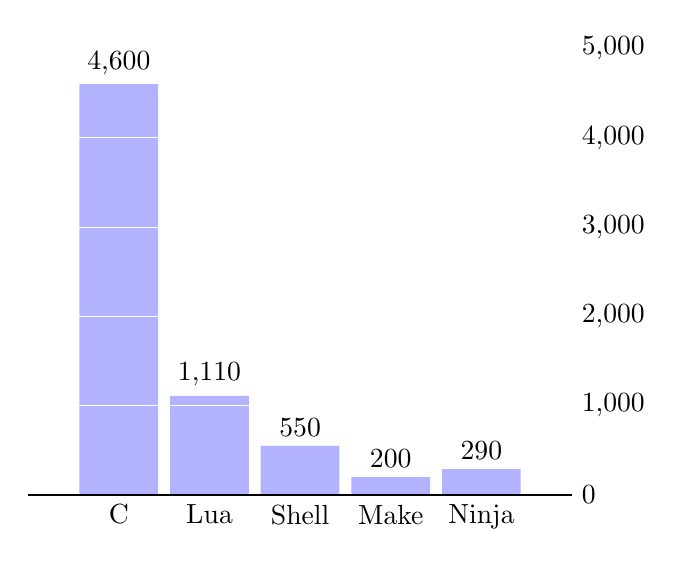
\begin{tikzpicture}
		\begin{axis}[
			style={/pgf/number format/assume math mode=true},
			width=0.7\textwidth,
			ybar, axis on top,
			ymajorgrids, tick align=inside,
			major grid style={draw=white},
			enlarge y limits={value=.1,upper},
			axis x line*=bottom,
			axis y line*=right,
			y axis line style={opacity=0},
			enlarge x limits=0.25,
			tickwidth=0pt,
			xtick=data,
			bar width=1cm,
			symbolic x coords={C, Lua, Shell, Make, Ninja},
			nodes near coords,
			ymin=0,
			]
			\addplot[draw=none, fill=blue!30] coordinates {
				(Lua,1110) (C,4600) (Shell,550) (Make,200) (Ninja,290)
			};
		\end{axis}
	\end{tikzpicture}
	\caption{Lines of code in \Eol*, per language.}
	\label{fig:eol-loc}
\end{figure}

Last but not least, the \Eol* FFI module has been tested thoroughly, in two
ways:

\begin{itemize}

	\item With an automated test suite, which can be used for regression
	testing—and has been used as such to ensure that the behaviour of code
	generated by the JIT compilation of function invocations works the same
	way as the \verb|libffi|-based method.

	\item Writing example programs which exercise the module. These use third
	party libraries used in real world projects, so the example programs
	stress the FFI in the way it is intended to be used.

\end{itemize}

\section{Lessons Learned}

During the development of the project, the specification of the ELF and DWARF
standards has been analyzed, and the relevant parts which are useful for
implementing a \gls{FFI} have been identified. A comprehensive understanding
of the specification was acquired thanks to the following documentation:

\begin{itemize}

	\item \emph{How Debugging Works}~\cite{howdebugworks}: Tutorial-style
	series of articles which give a good overall overview of how debugging
	information is embeeded into compiled object code.

	\item \emph{System V Application Binary Interface Edition
	4.1}\cite{elfspec-sysv}: Contains the original (non normative)
	  specification of the ELF object file format. Though newer, normative
	  versions of the specification exist, this version explains the concepts
	  needed to understand the DWARF debugging information in an more
	  approachable way.

	\item \emph{DWARF Debugging Information Format Version
	4}~\cite{dwarfspecv4}: Normative specification of the DWARF debugging
	  information format.

\end{itemize}

Existing FFI implementations for Lua have been analyzed to understand how they
work, which was a valuable knowledge to keep in mind while designing how \Eol*
bridges native code to Lua. In particular, the LuaJIT \verb|ffi| module was
taken as a prime example of a proven solution which is popular in the Lua
community. The following documents were instrumental for the design of the
developed solution:

\begin{itemize}

	\item \emph{FFI semantics}~\cite{lj-ffi-semantic}: Describes how the
	module interacts both with Lua, and the compiled C code.

	\item \emph{ffi.* API functions}~\cite{lj-ffi-api}: Describes the API
	of the \verb|ffi| module.

\end{itemize}

Implementing the JIT code generation required learning how to use LuaJIT's
DynASM, which lacks official documentation. It was also needed to learn to
program in assembler for the Intel x86 platform, and its \gls{ABI} calling
conventions during the development of the JIT code generator.


\section{Planning Results}

\begin{table}[ht]
	\centering
	\begin{tabular}{rlrrrr}
		\toprule
		& & \multicolumn{2}{c}{Time (days)} & \multicolumn{2}{c}{Cost (€)} \\
		\cmidrule(r){3-6}
		\# & Task & Estimated  & Actual  & Estimated & Actual \\
		\midrule
		1. & Initial study     & 10 &  5 &  5.200 &  2.600 \\
		2. & Analysis          & 15 & 23 &  7.800 & 11.960 \\
		3. & Development       & 50 & 80 & 26.000 & 41.600 \\
		4. & Validation        & 10 &  8 &  5.200 &  4.160 \\
		5. & Documentation     & 30 & 78 & 15.600 & 40.560 \\
		\midrule
		  & \emph{Total}      & 115 & 194& 59.800 & 100.880 \\
		\bottomrule
	\end{tabular}
	\caption{Estimated vs.\ actual schedule and cost}
	\label{tab:sched-postmortem}
\end{table}

The planning done \emph{a priori} (\autoref{sec:plan-method}) resulted in a
tight schedule which did not include enough clearance for anything else than
the smallest of the unexpected delays~(c.f \autoref{tab:sched-postmortem}).
In hindsight, it would have been good to schedule additional time to cope
with the multiple causes of delays:

\begin{itemize}

	\item The main deviation, filed under \emph{Documentation}, was caused
	because the effort of writing the final report was underestimated by
	a wide margin. The estimation was overly optimistic, and while for someone
	used to do documentation work in a regular basis it might have been an
	adequate estimation, that was not the case for the author. Plus, there was
	the added difficulty of writing the documentation in English: while
	capable of its fluent use in a daily basis, the author is not a native
	speaker and lacked experience in writing long-form technical documentation
	in it.

	\item The additional time needed for the \emph{Analysis} was motivated by
	the need of reading complex normative documentation, mainly the
	specifications of the \gls{ELF} and \gls{DWARF} standards, which weight
	over 320 and 100 pages, respectively. Even though not the whole text of
	the specifications was relevant for the present project, it was needed to
	wade through them to acquire concepts which then allowed to understand the
	rest.

	\item As for the \emph{Development} phase, it took a good amount of
	unplanned time to understand how use DynASM for JIT code generation due to
	the utter lack of documentation, which required frequent detours to read
	parts of its source code. The most complete resource on
	DynASM~\cite{unofficial-dasm-doc} was written by a third party, it is not
	part of official documentation, and it was found when the most of the
	deviation had already taken place.

\end{itemize}


On the other side of the spectrum, the \emph{Initial study} was carried out
faster than planned: the preexisting knowledge about Lua, LuaJIT, and the
existing solutions to use native libraries with them was a valuable asset.

The final cost of the project has increased accordingly to the additional time
needed for its completion, being now 100.800€ instead of the planned 59.800€.
This figure does not take into account the time devoted by the tutor of the
project.


\section{Future Directions}

Every software project has room for improvement and continued refinement, and
\Eol* is no exception. There are a number of features which have been
knowingly left out of the present project, in order to keep its scope under
control. It is the intention of the author to keep developing \Eol* as a Free
Software project, and there are a number of ideas for future development which
have surfaced during the realization of its current version.

The following are ideas which are complex to realize, and even though working
on them would require a big development effort, they open the path to exciting
new possibilities:

\begin{itemize}

	\item Defining an on-disk format for type and function information. The
	idea would be to obtain the information from the DWARF debugging
	information, and store it in a format which is optimized for faster
	reading. The files in this new format would be used for on-disk caching.

	\item Using the file format implemented from the previous bullet point,
	allow reading type information directly from it, without requiring that
	the ELF shared objects include DWARF debugging information.

	\item Saving the generated code to disk in ELF object files, when \Eol* is
	built with JIT code generation enabled.	The generated code could be loaded
	reusing the Lua module loader.

	\item Implementing support for reading debugging information in formats
	other than DWARF. Ideally, there would be an interface that a “type
	information provider” component could implement, and the DWARF provider
	would be just one of many.

\end{itemize}

The following fall into the category of improvements which can be done with
a moderate effort, and would certainly provide added value to the project:

\begin{itemize}

	\item Building a community. \Eol* is already Free Software, it lacks
	a community, and it would be interesting to foster a healthy one around
	the project. That would require writing more documentation (e.g. a quick
	start tutorial, a walkthough of the features), and having public
	communication channels (e.g. a mailing list, an \gls{IRC} chat room,
	participating in the \verb|lua-l| list...).

	\item Ensuring compatibility. Making sure that \Eol* works with Lua 5.2,
	and	5.1 would favour maximum adoption, since those are the versions more
	widely deployed.\todo{See if it's possible to add a citation}

	\item Enabling use of \Eol* with LuaJIT. Most modules using the Lua C API
	can be built for LuaJIT as well. LuaJIT is designed to be compatible with
	Lua	5.1, while the current Implementation targets version 5.3.

	\item Implementing JIT compilation of function invocations for
	architectures other than x86, and x86\_64. This can be done with ease for
	the other architectures supported by DynASM: ARM, MIPS, and PowerPC.

\end{itemize}

\beforeintro
